\documentclass[11pt]{article}
\usepackage{fullpage,amsthm,amsfonts,amssymb,epsfig,amsmath}
\usepackage{listings}
\usepackage{color}
\usepackage{graphicx}

\definecolor{dkgreen}{rgb}{0,0.6,0}
\definecolor{gray}{rgb}{0.5,0.5,0.5}
\definecolor{mauve}{rgb}{0.58,0,0.82}

\lstset{frame=tb,
  language=Java,
  aboveskip=3mm,
  belowskip=3mm,
  showstringspaces=false,
  columns=flexible,
  basicstyle={\small\ttfamily},
  numbers=none,
  numberstyle=\tiny\color{gray},
  keywordstyle=\color{blue},
  commentstyle=\color{dkgreen},
  stringstyle=\color{mauve},
  breaklines=true,
  breakatwhitespace=true,
  tabsize=3
}

\begin{document}

\noindent Abhishek Gupta

\vspace{2mm}

\noindent CMPS 102

\vspace{2mm}

\noindent Homework 5

\vspace{2mm}

\noindent 12 May 2015

\vspace{2mm}

\centerline{Homework 5}

\vspace{2mm}

\noindent In all problems address the following:

\textbf{a)} What subproblems are you solving?

\textbf{b)} How are the subproblem related?

\textbf{c)} Give a recurrence What is the precise meaning of the entries of the recurrence?

\textbf{d)} What table are you filling in in what order?

\textbf{e)} How is the table initialized?

\textbf{f)} An arrow diagram for the recurrence

\textbf{g)} Time bound with justification

\vspace{2mm}

\noindent \textbf{PROBLEM 0:}

\vspace{2mm}

\noindent A rabbit wants to go through a distance of n feet. It can either do a short hop of one foot or a long hop of three feet. Denote f(n) as the number of ways that the rabbit can go through a distance of n feet. 

\noindent For instance, if n=5 we have the ways below:

1. short - short - short - short - short

2. long - short - short

3. short - long - short  

4. short - short - long

\noindent Thus f(5)=4. Give an O(n) algorithm to find f(n).

\vspace{6mm}

\noindent \textbf{PROBLEM 1:} 

\vspace{2mm}

Let $G = (V, E)$ be an undirected graph with $n$ nodes.  Recall that a subset of the nodes is called an independent set if no two of them are joined by an edge. Finding large independent sets is difficult in general; but here we'll see that it can be done efficiently if the graph is ``simple'' enough. 

Call a graph $G = (V, E)$ a path if its nodes can be written as $v_1, v_2, ...,v_n$, with an edge between vi and $v_j$ if and only if the numbers $i$ and $j$ differ by exactly 1. With each node $v_i$, we associate a positive integer weight $w_i$. 

Consider, for example, the five-node path drawn in Figure 6.28. The weights are the numbers drawn inside the nodes. 

The goal in this question is to solve the following problem:

\vspace{2mm}

\emph{Find an independent set in a path G whose total weight is as large as possible.}

\vspace{2mm}

\noindent \textbf{(a)} Give an example to show that the following algorithm does not always find an independent set of maximum total weight.

\begin{lstlisting}
The "heaviest-first" greedy algorithm 
	Start with S equal to the empty set 
	While some node remains in G 
		Pick a node vi of maximum weight 
		Add vi to S 
		Delete vi and its neighbors from G 
	Endwhile 
	Return S
\end{lstlisting}

\noindent \textbf{(b)} Give an example to show that the following algorithm also does not always find an independent set of maximum total weight.

\begin{lstlisting}
Let S1 be the set of all vi where i is an odd number 
Let S2 be the set of all vi where i is an even number 
(Note that S1 and S2 are both independent sets) Determine which of S1 or S2 has greater total weight, and return this one

\end{lstlisting}

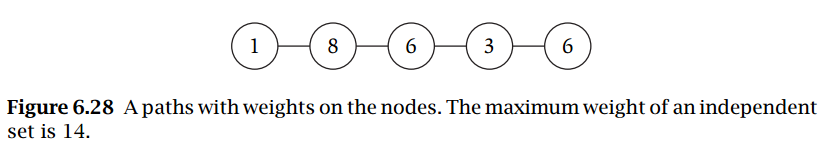
\includegraphics[scale=0.75]{1.png}

\vspace{2mm}

\noindent \textbf{(c)}  Give an algorithm that takes an n-node path G with weights and returns an independent set of maximum total weight. The running time should be polynomial in n, independent of the values of the weights.

\vspace{6mm}

\noindent \textbf{PROBLEM 2:} 

\vspace{2mm}

\noindent Let $G = (V, E)$ be a directed graph with nodes $v_1, ..., v_n$. We say that G is an ordered graph if it has the following properties. 

\vspace{2mm}

\textbf{(i)} Each edge goes from a node with a lower index to a node with a higher index. That is, every directed edge has the form $(v_i, v_j)$ with $i < j$. 

\vspace{2mm}

\textbf{(ii)} Each node except vn has at least one edge leaving it. That is, for every node $v_i$, $i = 1, 2, ..., n − 1$, there is at least one edge of the form $(v_i,v_j)$. 

\vspace{2mm}

The length of a path is the number of edges in it. The goal in this question is to solve the following problem (see Figure 6.29 for an example).

\vspace{2mm}

\emph{Given an ordered graph G, find the length of the longest path that begins at $v_1$ and ends at $v_n$.}

\vspace{2mm}

\noindent \textbf{(a)} Show that the following algorithm does not correctly solve this problem, by giving an example of an ordered graph on which it does not return the correct answer.

\begin{lstlisting}
Set w = v_1
Set L = 0

While there is an edge out of the node w 
	Choose the edge (w, v_j) 
		for which j is as small as possible 
	Set w = v_j 	
	Increase L by 1 
end while 
Return L as the length of the longest path

\end{lstlisting}

\vspace{2mm}

In your example, say what the correct answer is and also what the algorithm above finds.

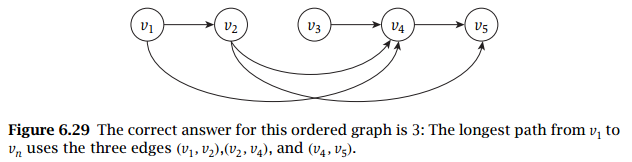
\includegraphics[scale=1]{2.png}

\vspace{2mm}

\noindent \textbf{(b)} Give an efficient algorithm that takes an ordered graph G and returns  the length of the longest path that begins at $v_1$ and ends at $v_n$.(Again, the length of a path is the number of edges in the path.)

\vspace{6mm}

\noindent \textbf{PROBLEM 3:} 

\vspace{2mm}

\noindent In a word processor, the goal of ``pretty-printing'' is to take text with a ragged right margin, like this,

\vspace{2mm}

\begin{lstlisting}
Call me Ishmael. 
Some years ago, 
never mind how long precisely,
having little or no money in my purse, 
and nothing particular to interest me on shore, 
I thought I would sail about a little 
and see the watery part of the world.

\end{lstlisting}

\vspace{2mm}

\noindent and turn it into text whose right margin is as ``even'' as possible, like this.

\vspace{2mm}

\begin{lstlisting}

Call me Ishmael. Some years ago, never 
mind how long precisely, having little 
or no money in my purse, and nothing 
particular to interest me on shore, I 
thought I would sail about a little 
and see the watery part of the world.

\end{lstlisting}

\vspace{2mm}

To make this precise enough for us to start thinking about how to write a pretty-printer for text, we need to figure out what it means for the right margins to be ``even.'' So suppose our text consists of a sequence of words, $W={w_1,w_2,...,w_n}$, where $w_i$ consists of $c_i$ characters. We have a maximum line length of L. We will assume we have a fixed-width font and ignore issues of punctuation or hyphenation. 

A formatting of W consists of a partition of the words in W into lines. In the words assigned to a single line, there should be a space after each word except the last; and so if $w_j, w_{j+1}, ..., w_k$ are assigned to one line, then we should have 

\centerline{ $\displaystyle[\sum_{i = j}^{k - 1} (c_i + 1)] + c_k \le L.$
}

\noindent We will call an assignment of words to a line valid if it satisfies this inequality. The difference between the left-hand side and the right-hand side will be called the slack of the line—that is, the number of spaces left at the right margin. 

Give an efficient algorithm to find a partition of a set of words W into valid lines, so that the sum of the squares of the slacks of all lines (including the last line) is minimized.

\vspace{6mm}

\noindent \textbf{PROBLEM 4:} 

\vspace{2mm}

\emph{Gerrymandering} is the practice of carving up electoral districts in very careful ways so as to lead to outcomes that favor a particular political party. Recent court challenges to the practice have argued that through this calculated redistricting, large numbers of voters are being effectively (and intentionally) disenfranchised. 

Computers, it turns out, have been implicated as the source of some of the ``villainy'' in the news coverage on this topic: Thanks to powerful software, gerrymandering has changed from an activity carried out by a bunch of people with maps,pencil,and paper into the industrial-strength process that it is today. Why is gerrymandering a computational problem? There are database issues involved in tracking voter demographics down to the level of individual streets and houses; and there are algorithmic issues involved in grouping voters into districts. Let's think a bit about what these latter issues look like. 

Suppose we have a set of n precincts $P1, P2, ..., Pn$, each containing m registered voters. We're supposed to divide these precincts into two districts, each consisting of $n/2$ of the precincts. Now, for each precinct, we have information on how many voters are registered to each of two political parties. (Suppose, for simplicity, that every voter is registered to one of these two.) We'll say that the set of precincts is susceptible to gerrymandering if it is possible to perform the division into two districts in such a way that the same party holds a majority in both districts.

Give an algorithm to determine whether a given set of precincts is susceptible to gerrymandering; the running time of your algorithm should be polynomial in $n$ and $m$. 

\vspace{2mm}

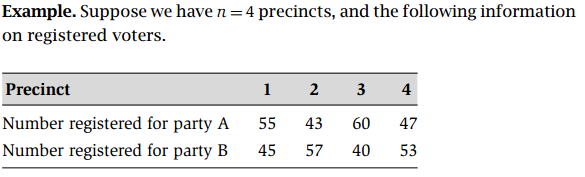
\includegraphics[scale=0.75]{3.png}

\vspace{2mm}

This set of precincts is susceptible since, if we grouped precincts 1 and 4 into one district, and precincts 2 and 3 into the other, then party A would have a majority in both districts. (Presumably, the ``we'' who are doing the grouping here are members of party A.) This example is a quick illustration of the basic unfairness in gerrymandering: Although party A holds only a slim majority in the overall population (205 to 195), it ends up with a majority in not one but both districts.

\vspace{6mm}

\noindent \textbf{PROBLEM 5: }

\vspace{2mm}

Recall the scheduling problem from Section 4.2 in which we sought to minimize the maximum lateness. There are $n$ jobs, each with a deadline $d_i$ and a required processing time $t_i$, and all jobs are available to be scheduled starting at time $s$. For a job $i$ to be done, it needs to be assigned a period from $s_i \ge s$ to $f_i = s_i + t_i$, and different jobs should be assigned nonoverlapping intervals. As usual, such an assignment of times will be called a schedule. 

In this problem, we consider the same setup, but want to optimize a different objective. In particular, we consider the case in which each job must either be done by its deadline or not at all. We'll say that a subset J of the jobs is schedulable if there is a schedule for the jobs in J so that each of them finishes by its deadline. Your problem is to select a schedulable subset of maximum possible size and give a schedule for this subset that allows each job to finish by its deadline. 

\vspace{2mm}

\noindent \textbf{(a)} Prove that there is an optimal solution $J$ (i.e., a schedulable set of maximum size) in which the jobs in $J$ are scheduled in increasing order of their deadlines. 

\vspace{2mm}

\noindent \textbf{(b)} Assume that all deadlines $d_i$ and required times $t_i$ are integers. Give an algorithm to find an optimal solution. Your algorithm should run in time polynomial in the number of jobs $n$, and the maximum deadline $D = max_i d_i$. 

\end{document}